\documentclass[10pt,a4paper]{report}
\usepackage{listings}
\usepackage{color}
\usepackage{graphicx}
\usepackage{fullpage}
\usepackage{subfigure}

\begin{document}

% Colors used by js Builder 3.
\definecolor{jspurple}{rgb}{0.55, 0.0, 0.55}
\definecolor{jsred}{rgb}{0.65, 0.01, 0.01}
\definecolor{jsgreen}{rgb}{0, 0.85, 0}
\definecolor{jsgray}{rgb}{0.25, 0.37, 0.75}
\definecolor{jsblue}{rgb}{0, 0.2, 1}
\definecolor{jsfunction}{rgb}{0.2, 0.6, 0.4}
\definecolor{jsvar}{rgb}{0.4, 0.6, 0.8}
\definecolor{white}{rgb}{1, 1, 1}
\definecolor{backgrnd}{rgb}{0.95, 0.95, 0.95}

% Define new language for listings.
\lstdefinelanguage{JavaScript}
{
	morekeywords={\colon},
	keywordstyle=\color{red},
	morekeywords={this, new, extends, implements, void, true, false, as, if, function, var},
	keywordstyle=\color{jspurple}\textbf,
	basicstyle=\ttfamily\scriptsize,
	sensitive=true,
	morecomment=[l][\color{jsgreen}\ttfamily]{//},
	morecomment=[s][\color{jsgreen}\ttfamily]{/*}{*/},
	morecomment=[s][\color{jsgray}\ttfamily]{/**}{*/},
	morestring=[b]",
	morestring=[b]',
	stringstyle=\color{jsblue}\textbf,
	commentstyle=\color{jsgreen},
	showstringspaces=false,
	numberstyle=\scriptsize,
	numberblanklines=true,
	showspaces=false,
	breaklines=true,
	showtabs=false,
	numbers=left,
	tabsize=2
}

\lstset {
    basicstyle=\footnotesize,      % font size
    numbers=none,                  % where to put line numbers
    numberstyle=\footnotesize,     % numbers size
    numbersep=5pt,                 % how far the line numbers are from the code
    backgroundcolor=\color{backgrnd}, % background color
    showspaces=false,                          % show spaces (with underscores)
    showstringspaces=false,            % underline spaces within strings
    showtabs=false,                            % show tabs using underscores
    frame=single,                  % adds a frame around the code
    tabsize=4,                     % default tabsize
    breaklines=true,                  % automatic line breaking
    columns=fullflexible,
    breakautoindent=false,
    framerule=1pt,
    xleftmargin=0pt,
    xrightmargin=0pt,
    breakindent=0pt,
    resetmargins=true
}

\lstset{language=JavaScript}

\title{Zarafa Webaccess 7.0 Design Document}
\date{November 18, 2009}
\author{Niels Brouwers}
	
\maketitle
\clearpage
        
\tableofcontents

\setlength{\parindent}{0.0in}
\setlength{\parskip}{0.1in}

\chapter{Introduction}

Zarafa provides an open source drop-in replacement for Microsoft Exchange Server, a messaging and groupware 
server product whose main features include e-mail, calendaring, and management of tasks and contacts. 
End users run a client application that connects to Exchange, most notably Microsoft Outlook or the web based
Outlook Web Access. Figure \ref{figure:stackms} shows the Microsoft messaging stack and how its products,
Exchange, Outlook, and Outlook Web Access relate to each other.

Zarafa offers alternatives to both Exchange Server and it's web access component. The Zarafa stack is 
shown in figure \ref{figure:stackzarafa}. End users of a Zarafa installation may either keep using 
Outlook (left) or choose to use the Zarafa Web Access (right). 

Evolution of browser technology, expressed in pervasiveness of new standards and improvements in
performance, have made it possible to build responsive and visually rich web applications with a 
'desktop' look and feel. Furthermore, open source libraries such as YUI and ExtJS significantly simplify
this task by providing a user interface framework with a rich set of standard components. 
Building on these new technologies, it is our ultimate ambition to build a web based alternative to 
not just Outlook Web Access, but also Outlook itself. 

This design document describes the architecture and implementation details of Zarafa's new web access.
Chapter \ref{section:ui} and \ref{section:communication} describe the user interface and communication 
protocols respectively. Chapter \ref{section:style} deals with code style and documentation practices.
Finally Chapter \ref{section:cookbook} contains detailed descriptions to show developers how to 
accomplish common tasks within our framework.

\begin{figure}[h!]
\centering
\subfigure[Microsoft]
{
	\includegraphics[width=7.5cm]{figures/stack_microsoft.eps}
	\label{figure:stackms}
}
\subfigure[Zarafa]
{
	\includegraphics[width=7.5cm]{figures/stack_zarafa.eps}
	\label{figure:stackzarafa}
}
\caption{Comparison of messaging software stacks.}
\label{figure:mszarafacomparison}
\end{figure}

\chapter{User interface}
\label{section:ui}

The application can be seen as a replacement for Exchange's web access, but also Outlook itself. When our
customers move from Microsoft's offering to Zarafa they want the transition to be as smooth as possible for
their end users. By providing an application that looks and feels like Outlook we minimise the learning 
curve for users, stimulating quick adoption.

\section{Overview}

The meat of the work is in developing a flexible user interface that presents \emph{items} (mail messages, 
appointments, tasks, contacts) to the user and lets the user create, manipulate, and exchange items with 
other users. There are three important aspects of the application that stimulate a high level of flexibility
and decoupling. 

\begin{itemize}
	\item{Outlook is a highly volatile application, 
	whose user interface changes radically at each major version. In order to keep up with new features added 
	to Outlook in the future, and to be able to add novel features of our own it is crucial that the interface
	architecture is not resistant to change and expansion.}
	\item{The application manages a variety of item types. 
	The application components that deal with these types have a low amount of interdependency, which
	makes it natural to develop them individually and concurrently.}
	\item{One of the requirements for the application is that it should be possible, and preferably easy,
	to develop third-party plug-ins.}
\end{itemize}

Ideally the application should be a loosely coupled group of components, where each component implements a sub-set 
of the functional requirements. We divide up the application into chunks called \emph{contexts}, each dealing with
a different entity type. Examples of contexts are the mail context, the calendar context, etc. This decoupling 
makes it possible to develop contexts independently on top of a global framework. The architecture is shown 
in Figure \ref{figure:architecture}.

\begin{figure}[h!]
\centering
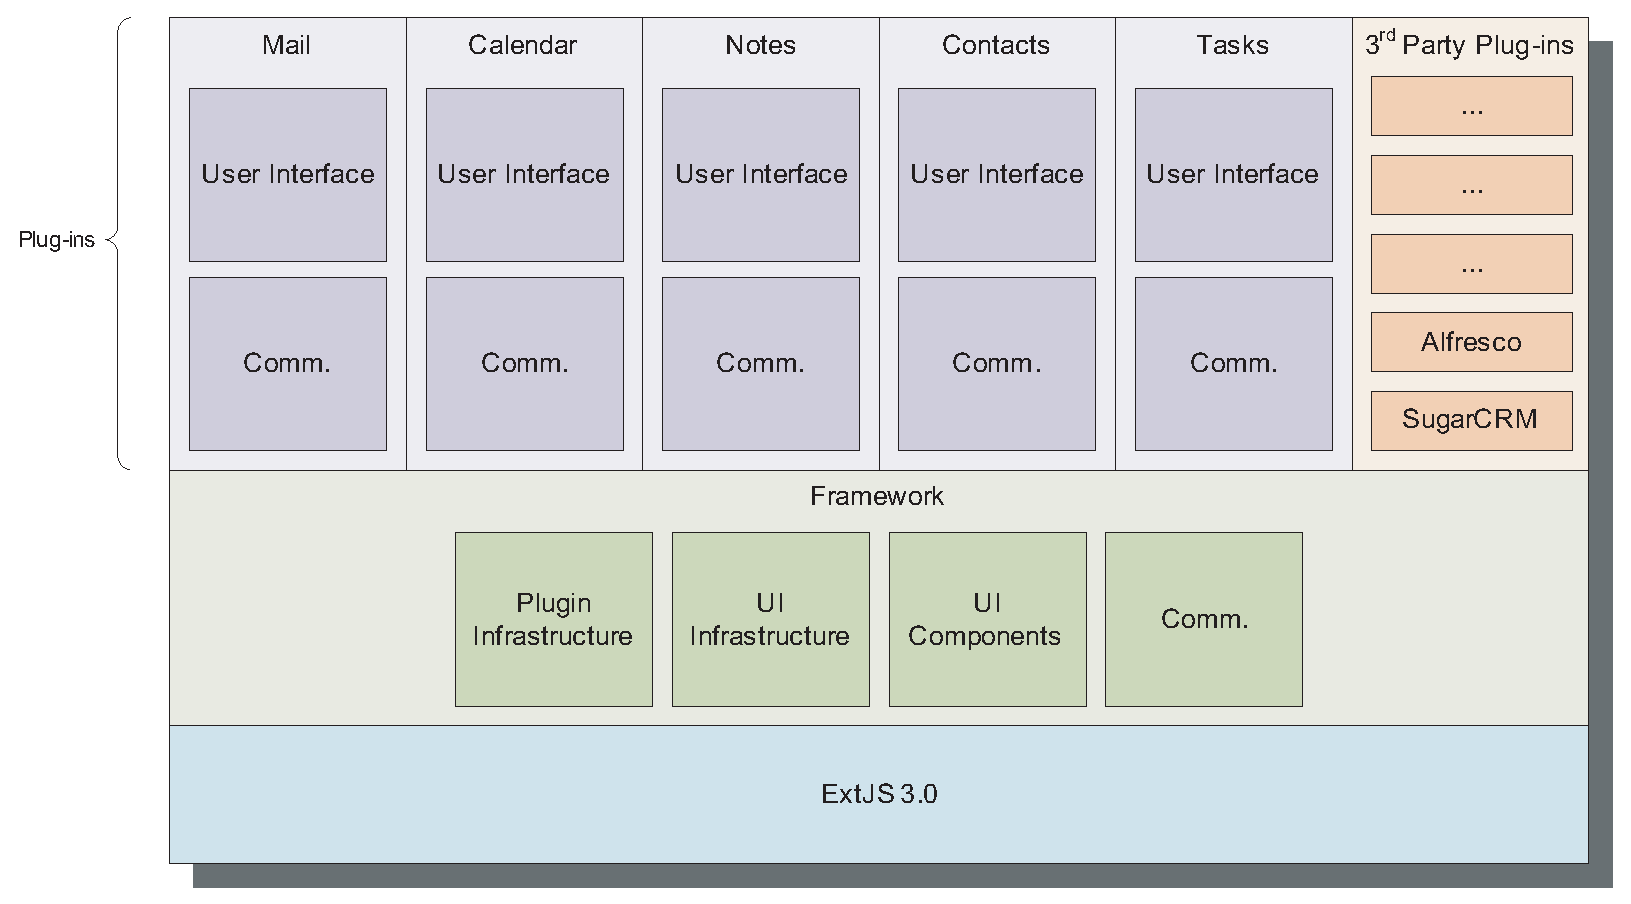
\includegraphics[width=14cm]{figures/stack.eps}
\caption{Architecture overview.}
\label{figure:architecture}
\end{figure}

The application framework sits atop the ExtJS 3.0 library and provides all the functionality that is needed across
contexts. The framework supports \emph{plug-ins}, functional components that can be added or removed at will. 
Contexts are implemented as plug-ins, and third-party developers can also develop their own to extend or 
customise the application.

The framework also provides a user interface infrastructure, with a main screen that carries all the standard
components that are used by all contexts. A set of custom user interface widgets such as a sophisticated
calendaring component are also included. Finally the framework supplies a communications API that allows
for both low-level and high-level interaction with the server-side back-end.

\section{Plug-ins}

The purpose of plug-ins is to have a way to add functionality to the application simply by adding additional
JavaScript files. 
Registered plug-ins can hook into so called \emph{insertion points} in the interface and register component
creation functions with them. This allows for a plug-in developer to easily add UI components such as buttons
or menu options to the application without modifying any 'core' code. 

A global object called {\tt container} manages, among other things, plug-ins. Plug-ins must extend {\tt Zarafa.ui.Plugin} 
and register a single instance with the container in order to be able to function. Plug-ins have unique names, by which
they can be identified and retrieved. 

Listing \ref{listing:exampleplugin} shows a bare-bones example plug-in. A new instance of the plug-in is created and
registered with the container on the last line of the code, using the {\tt registerPlugin} function. 
Note that the name of the plugin is a property of the
plugin itself, so there is no need to pass it when registering.

\begin{lstlisting}[caption={Example plugin.}, label=listing:exampleplugin]
// Ensure the 'Zarafa.plugins' namespace is declared.
Ext.namespace('Zarafa.plugins');

// Declare Zarafa.plugins.ExamplePlugin class.
Zarafa.plugins.ExamplePlugin = function()
{
	// Call parent constructor. Set plug-in name to 'example'.
	var config = { name : 'example' };
	Zarafa.plugins.ExamplePlugin.superclass.constructor.call(this, config);
};

// Express that the ExamplePlugin extends Plugin.
Ext.extend(Zarafa.plugins.ExamplePlugin, Zarafa.ui.Plugin, {
	
});

// Register a new instance of the plugin with the global container.
container.registerPlugin(new Zarafa.plugins.ExamplePlugin());\end{lstlisting}

\section{Contexts}
\label{section:contexts}

As discussed, functionality for working with different item types is encapsulated
in various contexts. Each context is a special type of plug-in that has additional functionality allowing it to 
'take over' the toolbar and main content section of application screen. Folders in the folder hierarchy are 
linked to contexts that display their contents, so that when a user clicks his or her inbox, the mail context
is enabled. 

The main application screen consists of several standard areas, shown in Figure \ref{figure:layout}.
The UI provides a standard hierarchy panel showing a list of folders the user has access to, as well as a 
bottom tool bar. Each context has its own content panel and tool bar, but only the ones belonging to the 
currently active context are visible while all others are hidden. This is achieved by loading the tool bars 
and content panels of all contexts into their respective areas and using card layouts to switch between them.

\begin{figure}[h!]
\centering
\includegraphics[width=10cm]{figures/layout.eps}
\caption{Screen layout.}
\label{figure:layout}
\end{figure}

Generally a context switch is performed when the user selects a folder from the hierarchy tree at the left
of the screen. A simple bidding mechanism is in place to determine which context will be used to show that
folder. Each content context implements a {\tt bid()} method that is passed store and folder details and
returns a numerical value indicating how well it is able to handle that folder type. The content context
that bids the highest is then selected.

\section{Insertion points}
\label{section:insertionpoints}

An \emph{insertion point} is a named location in the UI component hierarchy where plug-ins may add components. 
Insertion points are typically added to tool bars and context menus, and are intented as easy hooks for adding 
new buttons or menu items.

Plug-ins register functions with insertion points. When the application starts and the UI is constructed, 
these functions will be called automatically. They may return one or more UI components, which will be added 
to the hierarchy at the appropriate locations.

\subsection{Creating insertion points}

Insertion points are implemented as a call to the container, which collects UI components from registered
plug-ins and returns them. Listing \ref{listing:insertionpoints} shows how to create an insertion point. 

\begin{lstlisting}[caption={Insertion point.}, label=listing:insertionpoints]
function createToolbar()
{

	return new Ext.Toolbar(
	{

		items : [
				{
					iconCls : 'icon_delete',
				},
				{
					iconCls : 'icon_copy'
				},
				{
					iconCls : 'icon_print'
				},
				{
					iconCls : 'icon_addressbook'
				}, 
				'-',
				// insertion point 'example.toolbar'
				container.populateInsertionPoint('example.toolbar')
		]

	});
}
\end{lstlisting}

By design the names of the insertion points should reflect the structure of the application. Therefore
the proposed naming scheme follows a hierarchy separated by dot ('.') characters. For example, the
top tool bar of the 'tasks' context is called {\tt context.tasks.toolbar}. Insertion points may be contained 
in right-click menus (ie {\tt main.hierarchy.contextmenu}), dialogs (ie {\tt dialogs.properties.toolbar}),
and may even be nested.

Insertion points are supported by the documentation tool and should be documented for easy reference. More
on this in Section \ref{section:docinsert}.

\subsection{Using insertion points}

An example plug-in that adds a 'hello world' button to the toolbar is shown in Listing \ref{listing:exampleplugin2}. 
The plug-in registers the {\tt createButton} function with the {\tt example.toolbar} insertion point (line 9). 

\begin{lstlisting}[caption={Using an insertion point.}, label=listing:exampleplugin2]
Ext.namespace('Zarafa.plugins');

Zarafa.plugins.ExamplePlugin = function()
{
	config = { name : 'example' };
	Zarafa.plugins.ExamplePlugin.superclass.constructor.call(this, config);
	
	// register the 'createButton' method with the 'example.toolbar' insertion point.
	this.registerInsertionPoint('example.toolbar', this.createButton, this);
};

Ext.extend(Zarafa.plugins.ExamplePlugin, Zarafa.ui.Plugin, {
	
	// Creates a single button that pops up a 'Hello world!' message when clicked.
	createButton : function(insertionPoint)
	{
		return new Ext.Button({
			text : 'Hello!',
			handler : function()
			{
				alert('Hello world!');
			}
		});
	}	
	
});

container.registerPlugin(new Zarafa.plugins.ExamplePlugin());\end{lstlisting}

The function {\tt registerInsertionPoint(match, func, scope)} registers a function 'func' so that it is 
called when an insertion point 'match' is populated. The function should return one or more UI components
({\tt Ext.Component} instances). Note that the 'match' parameter can be either a {\tt string} denoting
the name of the insertion point, or a regular expression to match multiple insertion points.

It's possible to hook into several insertion points explicitly by registering each one separately,
or by using a regular expression. Listing \ref{listing:insertregexp} shows how the code from
Listing \ref{listing:exampleplugin2} could be altered to create a button on the tool bars
of all contexts. The match parameter has been changed to a regular expression that matches 
'context.mail.toolbar', 'context.notes.toolbar', etc.

\begin{lstlisting}[caption={Matching with regular expressions.}, label=listing:insertregexp]
this.registerInsertionPoint(/context\..*?\.toolbar/, this.createButton, this);\end{lstlisting}
 
\subsection{Parameters}

In some cases it's useful to have insertion points that provide extra information to the plug-in. An example 
is an insertion point in a context menu, where it's useful to pass the menu object ({\tt Ext.menu.Menu}) to the
creation function. Another example is a toolbar in a 'read mail' dialog, which might pass the entry ID of the 
item that is being shown to the plug-in. 

The modified insertion point declaration and button creation function are shown in Listing 
\ref{listing:insertionpoints2} and \ref{listing:exampleplugin3} respectively.

\begin{lstlisting}[caption={Insertion point with parameter.}, label=listing:insertionpoints2]
container.populateInsertionPoint('dialog.readmail.toolbar', mailEntryId);
\end{lstlisting}

\begin{lstlisting}[caption={Using an insertion point with parameters.}, label=listing:exampleplugin3]
createButton : function(insertionPoint, messageEntryId)
{
	return new Ext.Button({
		text : 'Hello!',
		handler : function()
		{
			alert('Message ID: ' + messageEntryId);
		}
	});
}	
container.registerPlugin(new Zarafa.plugins.ExamplePlugin());\end{lstlisting}






\chapter{Communication}
\label{section:communication}

The application is web based and communicates with the server back-end over HTTP. While the client is
a complete rewrite, the server side is taken from the legacy implementation. This section discusses
the protocols and APIs involved.

Section \ref{section:commoverview} gives a conceptual overview of how the client and server talk to 
each other and exchange messages. Section \ref{section:protocol} describes the XML protocol used, 
and section \ref{section:jsrequests} deals with issuing requests from JavaScript. Finally Section
\ref{section:stores} describes how \emph{stores}, server-backed data models that support CRUD 
operations, can be used to work with items on a high level.

\section{Conceptual overview}
\label{section:commoverview}

The back-end has a pluggable architecture, with functionality divided among a set of \emph{modules}.
Each module is a named entity, such as 'maillistmodule' or 'taskitemmodule', and exposes a specific
part of the Zarafa server functionality. The client communicates with a module by sending it one or 
more \emph{actions}. Each request may contain one or mode actions for one or more modules. Several 
modules may implement the same actions (such as 'list') so actions are grouped by target module.
The server processes each of the actions in sequence and formulates a response, also containing 
actions. The process is shown in Figure \ref{figure:messageexchange}. 

Although there is usually a one-to-one mapping between response actions and request actions, this does 
not neccesarily have to hold. As an example consider the situation in Figure \ref{figure:saveitem}.
In this exchange the client wants to create a new task and sends a {\tt save} action to the
{\tt tasklistmodule} on the server, as shown in Figure \ref{figure:saveitema}. If successful, the
module on the server responds with an {\tt item} action with information about the created task, such
as the generated entry ID, but it will also send a {\tt folderupdate} action containing updated 
information about the folder the item was created in. This last action is to notify the client that
there is now one more item in the folder. 

\begin{figure}[b!]
\centering
\includegraphics[width=8cm]{figures/message-exchange.eps}
\caption{A message exchange between the client and server.}
\label{figure:messageexchange}
\end{figure}

\begin{figure}
\centering
\subfigure[Client request.]
{
	\includegraphics[width=8cm]{figures/saveitemcomm1.eps}
	\label{figure:saveitema}
}
\subfigure[Server response.]
{
	\includegraphics[width=8cm]{figures/saveitemcomm2.eps}
	\label{figure:saveitemb}
}
\caption{Message exchange for creating a new item.}
\label{figure:saveitem}
\end{figure}

\section{Protocol}
\label{section:protocol}

Communication with the back-end starts with the client initiating a request. The data exchange format is
XML. As explained in the previous section, a request may contain multiple actions for multiple modules.

\begin{lstlisting}[caption={Client server communication: client request}, label=listing:clientrequest]
<?xml version="1.0" encoding="UTF-8"?>
<zarafa>
	<module name="maillistmodule" id="maillistmodule">
		<action type="list">
			<store>[store MAPI ID]</store>
			<entryid>[folder MAPI ID]</entryid>
		</action>
	</module>
</zarafa>
\end{lstlisting}

Listing \ref{listing:clientrequest} shows a minimal client request for listing mails in a folder. Parameters
to the action are nested inside the {\tt action} tag, and may contain a forest of key-value pairs. The
server will respond with a similarly constructed reply. 

\begin{lstlisting}[caption={Client server communication: server response}, label=listing:serverresponse]
<?xml version="1.0" encoding="UTF-8"?>
<zarafa>
	<module name="previewmailitemmodule" id="previewmailitemmodule">
		<action type="item">
			[mail item details would be included here]
		</action>
	</module>
	<module name="mailnotificationmodule" id="mailnotificationmodule">
		<action type="newitem">
			[mail item details would be included here]
		</action>
	</module>
</zarafa>
\end{lstlisting}

Listing \ref{listing:serverresponse} shows a possible response from the server. Note that the behavior of 
mail notifications is currently not implemented in the legacy back-end, but that this is a definite want-to-have 
feature for the future. It is merely used as an example of how the server might send back actions that are 
not immediate responses to actions issued in the request, like in the case of Figure \ref{figure:saveitem}.

\section{Submitting requests from Javascript}
\label{section:jsrequests}

To avoid having to construct XML requests manually all client requests are made through a global instance of the
{\tt Zarafa.comm.Request} class. This object provides JavaScript$\leftrightarrow$XML (de)serialisation, and allows 
other components to react to server actions via either events or callbacks.

Consider Listing \ref{listing:request}. A call is made to the request object (a global instance of which
can be obtained from the container using {\tt getRequest()}) to retrieve a single message. The first two 
arguments are the module name and action type, which are taken from enumeration objects 
{\tt Zarafa.comm.ModuleNames} and
{\tt Zarafa.comm.Actions} respectively. The third argument is a Javascript object containing the parameters
to the action, which in this case are the message's MAPI store Id and MAPI entry Id. 

\begin{lstlisting}[caption={Submitting a request}, label=listing:request]
container.getRequest().singleRequest(

	Zarafa.comm.ModuleNames.previewReadMailItem,
	Zarafa.comm.Actions.open,
	{
		store : storeId,
		entryid : entryId
	}
);
\end{lstlisting}

The parameter object is serialised into equivalent XML and embedded into the {\tt action} xml tag. The 
serialisation can become a little involved depending on the XML you want to create. Consider the example
in Listing \ref{listing:parameters1}, and the corresponding XML in Listing \ref{listing:parameters2}

\begin{lstlisting}[caption={Parameter serialisation, JavaScript}, label=listing:parameters1]
var parameters = {
		sort : {
			column : 'date_received'
		}
};
\end{lstlisting}

\begin{lstlisting}[caption={Parameter serialisation, XML}, label=listing:parameters2]
<sort>
	<column>date_received</column>
</sort>
\end{lstlisting}

This correspondence is straightforward and easy to work with. Unfortunately 'maillistmodule' expects the
'column' node to carry an XML attribute 'direction' which should be either 'asc' or 'desc', for ascending and
descending respectively. To accomodate this an alternative form lets you specify the column tag as an
object with a {\tt \_} property for the text node, and zero or more properties starting with {\tt \$} to
describe attributes. This is exemplified in Listings \ref{listing:parameters3} and \ref{listing:parameters4}.

\begin{lstlisting}[caption={Parameter serialisation, JavaScript}, label=listing:parameters3]
var parameters = {
		sort : {
			column : {
				_ : 'date_received'
				$direction : 'desc'				
			}
		}
};
\end{lstlisting}

\begin{lstlisting}[caption={Parameter serialisation, XML}, label=listing:parameters4]
<sort>
	<column direction="desc">date_received</column>
</sort>
\end{lstlisting}

\subsection{Callbacks}

As described in the previous section there are two ways for the client to respond to server actions.
One way is to pass callback functions to the {\tt singleRequest} method. This is shown in Listing 
\ref{listing:callbacks}.

\begin{lstlisting}[caption={Using callbacks}, label=listing:callbacks]
container.getRequest().singleRequest(
	Zarafa.comm.ModuleNames.previewReadMailItem,
	Zarafa.comm.Actions.open,
	{
		store : storeId,
		entryid : entryId
	},
	{
		item : function(response)
		{
			// do something with response.data
			alert(response.data.item.body);
		},
		error : function(error)
		{
			// do something with the error
			alert(error.message);
		}
	}
);
\end{lstlisting}

In this example a Javascript object is passed as an optional fourth argument to {\tt Response.singleRequest}.
The callback argument is a key/value set with named actions linked to JavaScript functions. In our example,
if the server responds to this request with an 'item' action, the corresponding function is fired and the
mail body is displayed. Note that this function will only be called in response to an 'item' action from
the module that this request is calling (the 'previewreadmailitemmodule' in this case). The callback
will be called with a {\tt Zarafa.comm.Response} object containing a module name, action type, and a data
object which encapsulates the response data from the server.

It is also possible hook an error callback, which will be called when something goes wrong. An error
object is passed into the callback with information about the type of error and a user-friendly error 
message.

\subsection{Events}

In some cases it is in the interest of low inter-object dependency (low coupling) to have objects respond
to server actions that are not a result of a request issued directly by themselves. Consider the case
described in Section \ref{section:protocol}, where new mail notifications are piggy-backed. It is undesirable
to use callbacks to handle the 'newitem' action for two reasons. First, every request may generate such an 
action from the server, so each and every request would need to have a 'newitem' callback function attached. 
Second, callbacks are hooked by action type, and only respond to server actions from the module that the 
request was meant for. 

To address these issues the {\tt Request} object supports events that can be tied to specific combinations
of modules and actions. This makes it possible to tie a handler to the 'newitem' action of the 
'mailnotificationmodule' in any point in the code. In our example the hierarchy tree may for instance want
to listen to such events so that it may visually update the number of unread items in the user inbox.
The process is illustrated in Listing \ref{listing:events}

\begin{lstlisting}[caption={Using callbacks}, label=listing:events]
container.getRequest().addListener(
	Zarafa.comm.ModuleNames.mailNotification,
	Zarafa.comm.Actions.newItem,
	function(response)
	{
		alert('You have new mail');
	}
);
\end{lstlisting}

A special event case is the error event which, like the callback, fires when a request fails. This event
can be used to catch errors at a global scope, for instance to present the user with the opportunity
to re-login when the session has timed out.

\section{Stores}
\label{section:stores}

A MAPI folder can be seen as a flat list of items, much like a table in a database. Instead of directly issuing
action requests from the client to list or mutate items, a high-level API is provided that exposes
a MAPI folder as an ExtJS \emph{store} ({\tt Ext.data.Store}). A store is a client-side cache of items that exist
on the server, and provides a clean interface for loading and CRUD operations. 

Many standard ExtJS components use stores to manage the data they display and operate on. In MVC terms,
a store is the default \emph{model} for many UI components. A common example is the grid panel 
({\tt Ext.grid.GridPanel}). Displaying a list of tasks in a tasks folder is a matter of constructing a 
store instance, initialising it with the proper parameters (store ID), and connecting it to the grid. The
grid will automatically issue a generic 'load' command to the store to populate it with data which
is then displayed. 

\begin{figure}[t!]
\centering
\includegraphics[width=14cm]{figures/store2.eps}
\caption{Data flow.}
\label{figure:stores}
\end{figure}

Figure \ref{figure:stores} how various components connect to get data from the server to display in a 
data grid in the browser. A grid panel is connected to a store, which acts as a local data base holding
a set of records. The store uses a proxy to talk to the server, which in turn tasks with a server-side
\emph{list module} using the communication scheme described in previous sections. The server has different 
list modules for each type of data (tasks, mail, etc), and there are corresponding stores and proxies on 
the client.

Stores can be constructed with a store- and folder MAPI id, or these can be passed explicitly to the 
load method. Please refer to Section \ref{section:taskscontext} for a code example of this principle
in action. However stores can do more than just plain data loading. They support pagination and sorting,
and it's very easy to get this to work with the standard ExtJS components.

Records can be added, removed, or updated. Changes made to the data in a store can be committed to the 
server by calling the {\tt save} method. 



\chapter{Style guidelines}
\label{section:style}

\section{Object oriented design}

The ExtJS toolkit was founded on a solid OO-inspired design, using classes and inheritance. The application
is developed using the same style as ExtJS, so that our code integrates well with existing ExtJS components.

To declare a new class, one usually starts with defining the constructor. It is customary, but not required, 
to have a 'configuration' object as the first parameter. Configuration parameters are object/value pairs 
that configure specific parts of an object's instantiation, avoiding large sparse parameter lists. The 
constructor calls the constructor of its parent manually (as there is no way of doing this automatically). 
Listing \ref{listing:declaringclass} shows an example of this process. 

\begin{lstlisting}[caption={Declaring a new class}, label=listing:declaringclass]
// Zarafa.ui.mail.PreviewPanel constructor
Zarafa.ui.mail.PreviewPanel = function(config)
{
	// call the parent constructor
	Zarafa.ui.mail.PreviewPanel.superclass.constructor.call(this, config);
};

// Zarafa.ui.mail.PreviewPanel extends Ext.Panel
Ext.extend(Zarafa.ui.mail.PreviewPanel, Ext.Panel);
\end{lstlisting}

The call to {\tt Ext.extend()} expresses that {\tt Zarafa.ui.mail.PreviewPanel} extends (is a child class of) 
{\tt Ext.Panel}. It is now possible to substitute an instance of the former for the latter. If the class 
you're writing is not a child class of anything, simply extend from {\tt Object}.
ExtJS offers a range of handy tools besides {\tt Ext.extend()} that help us write modular code.

\section{Architectural style}

\subsection{Namespaces}

The ExtJS toolkit provides the {\tt Ext.namespace} function that declares a namespace. We place chunks of
related functionality in namespaces and let the code tree reflect the namespace hierarchy. For example, classes
in the {\tt Zarafa.ui.mail} namespace are defined in Javascript files that can be found in {\tt zarafa/ui/mail}.

\subsection{Singletons}

Static functions can be declared inside an \emph{singleton} object. A singleton, in OO design, is a class which
only has a single instance. This can be easily simulated in Javascript. For example, consider Listing 
\ref{listing:singleton}.

\begin{lstlisting}[caption={Declaring a singleton.}, label=listing:singleton]
/**
 * @class Zarafa.comm.Mail
 * 
 * The Mail object is a singleton containing several convenience methods for working with email messages.
 * 
 * @singleton
 */
Zarafa.comm.Mail = 
{
	openMail : function(storeId, entryId, callBack, errorCallback)
	{
		// implementation goes here
	}
};
\end{lstlisting}

This creates a function {\tt openMail} in the {\tt Zarafa.comm.Mail} object, which can be called anywhere in the
code as {\tt Zarafa.comm.Mail.openMail()}. By putting static functions in a singleton, we can group such
functions and document them as a unit.

\subsection{Enums}

An enumeration, or \emph{enum} for short is an object that contains a set of constants. They can be 
implemented as a JavaScript object.

\begin{lstlisting}[caption={Declaring an enumeration}, label=listing:enum]
/**
 * @class Zarafa.comm.Appointment.BusyStatus
 * 
 * Enumerates the different busy status types. 
 * 
 * @singleton
 */
Zarafa.comm.Appointment.BusyStatus = 
{
	
	// property documentation omitted for clarity
	free : 0,
	tentative : 1,
	busy : 2,
	outOfOffice : 3
};
\end{lstlisting}

Listing \ref{listing:enum} shows the {\tt Zarafa.comm.Appointment.BusyStatus} enum, enumerating all possible
values the 'busy status' value an appointment may take.  Enums should be used to avoid so called 'magic numbers'
in code. 

\section{Code style}

To keep our sanity of ourselves and the people working on this project after us it's important to write code
that is both clear, simple, and uniform in style. 

\subsection{Naming}

Copying the convention from ExtJS, namespaces are all in lowercaps except for the Z in 'Zarafa' 
(ie {\tt Zarafa.ui.mail}). Classes are camelcase starting with uppercase ({\tt Zarafa.ui.mail.MailGridPanel})
and variables, methods, and fields are camelcase starting with lowercase ({\tt Zarafa.comm.Mail.openMail()}).

\subsection{Method length}

Generally when methods span many lines it is possible to break up the function is maller pieces. This increases
readability as the reader does not need to know exactly how each part of the function is implemented to understand
the general idea. Break up functions of more than 30-50 lines or so should be broken up into smaller ones if 
possible. 

\section{Documentation}
	
I would like to stress that any piece of code that is not documented \emph{is not done}. Please don't close
tickets on uncommented code. We use the {\tt ext-doc} documentation tool provided by the ExtJS people.

This documentation tool allows documentation of Javascript code much like Javadoc or Doxygen. This section
describes how to document your code.
Since Javascript is a very dynamic language it's pretty much impossible to detect class, method, and field
definitions, and the relationships between them. Therefore documenation is quite explicit and you have to
declare classes, methods, and fields manually. This section briefly describes the most important aspects
of documenting with ext-doc. Please refer to the ext-doc documentation wiki for more information.

\subsection{Documenting classes}

You declare a class using the {\tt @class} statement inside a {\tt /** */} multi-line comment. You can
use {\tt @extends} to indicate that the class is a subclass of another class. After these two statements
you can fill in a description of the class. Optionally you can use the {\tt @singleton} statement to declare 
the class a singleton. 
The constructor can be documented separately and is documented much like a method. Finally use {\tt @cfg}
to declare configuration options for this class. Note that parameters and configuration options are typed.
A full example is shown in Listing \ref{listing:classdoc}.

\begin{lstlisting}[caption={Declaring a new class}, label=listing:classdoc]
/**
 * @class Zarafa.ui.ContextContainer
 * @extends Ext.Container
 * [ Description goes here ]
 * @constructor
 * @parameter config configuration object
 * @cfg String name the name of the context container.
 * @cfg Ext.Component defaultItem a default component to be shown if a context does 
 * not provide a component for this ContextContainer. 
 */
Zarafa.ui.ContextContainer = function(config)
{
	Zarafa.ui.ContextContainer.superclass.constructor.call(this, config);
};
\end{lstlisting}

\subsection{Documenting methods}

Listing \ref{listing:methoddoc} shows how to document methods using the {\tt @method} tag. Parameters can be
specified using {\tt @param} with a type, name, and description. If an argument is optional please make
this explicit by using {\tt (optional)} as exemplified by the errorCallBack parameter in listing 
\ref{listing:methoddoc}.

\begin{lstlisting}[caption={Declaring a new class}, label=listing:methoddoc]
Zarafa.comm.Mail = 
{

	/**
	 * Opens a mail asynchronously.
	 * 
	 * @param {String} storeId a MAPI ID that corresponds to a MAPI store 
	 * @param {String} entryId a MAPI ID that corresponds to an item in the given store
	 * @param {Function} callback a function that will be called when the message has arrived 
	 *	from the server  
	 * @param {Function} errorCallback (optional) a function that will be called when an error 
	 *	occurred retrieving the mail
	 * @method openMail
	 */
	openMail : function(storeId, entryId, callBack, errorCallback)
	{
		// implementation
	}
	

};
\end{lstlisting}

\subsection{Documenting insertion points}
\label{section:docinsert}



\chapter{Cookbook}
\label{section:cookbook}

In this chapter the reader will learn about the webaccess architecture by example. 

\section{Folder details plugin}
\label{section:folderdetails}

Our first task is to write a simple plugin that shows the status of the currently selected folder.
As the user selects folders from the hierarchy tree on the left of the screen a line of text
in the bottom toolbar is updated, showing the number of total and unread items in the folder.
The screen shot in Figure \ref{figure:plugin} shows the component in action. The finished
implementation can be found in the source tree in {\tt Zarafa.plugins.FolderStatus}.

\begin{figure}[h!]
\centering
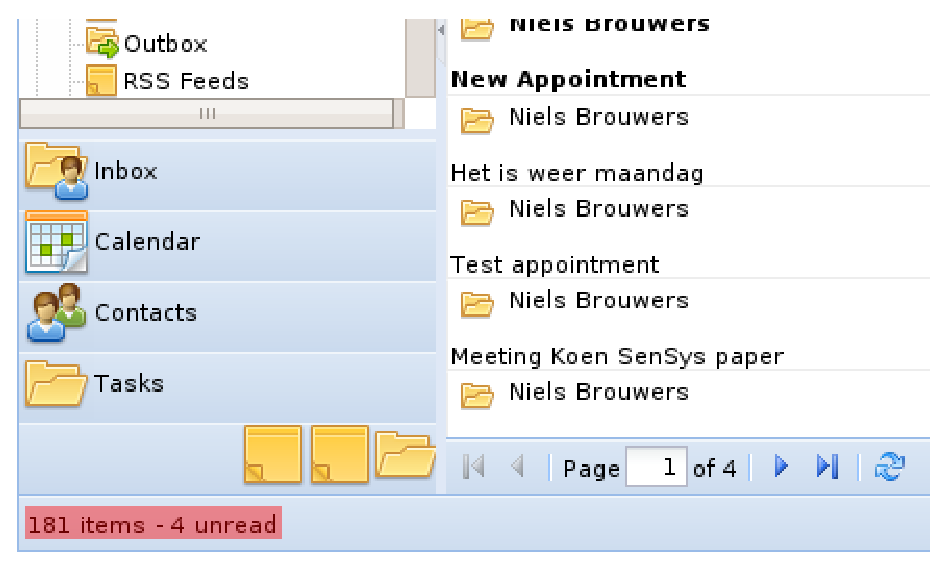
\includegraphics[width=9cm]{figures/plugin.eps}
\caption{Folder status plugin.}
\label{figure:plugin}
\end{figure}

We will start by writing some boilerplate, shown in Listing \ref{listing:plugin1}. The class 
{\tt Zarafa.plugins.FolderStatus} is declared, extending {\tt Zarafa.ui.Plugin}
\footnote{More info on OO and ExtJS can be found at http://www.extjs.com/learn/Manual:Intro}.
Each registered plug-in has a name, so the name 'folderstatus' is passed to the parent
constructor. On line 11 a single instance of this plugin is created and registered with the
global container. For convenience we add an {\tt init} method that is called right
after the parent constructor.

\begin{lstlisting}[caption={Plugin boilerplate}, label=listing:plugin1]
Zarafa.plugins.FolderStatus = function()
{
	config = { name : 'folderstatus' };
	Zarafa.plugins.FolderStatus.superclass.constructor.call(this, config);
	
	// Initialise the plug-in.
	init();
};

Ext.extend(Zarafa.plugins.FolderStatus, Zarafa.ui.Plugin, {

	init : function()
	{
		this.registerInsertionPoint('statusbar.left', this.createFolderStatus, this);
	},
	
	createFolderStatus : function(insertionPoint)
	{
		// Create a new toolbar text item.
		this.textItem = new Ext.Toolbar.TextItem({});
		this.textItem.setText('Hello World!');

		return this.textItem;
	}

});

container.registerPlugin(new Zarafa.plugins.FolderStatus());
\end{lstlisting}

In order to get something on screen we need to hook into an insertion point 
(see Section \ref{section:insertionpoints}). We hook into the {\tt statusbar.left} insertion
point, which is located on the bottom bar, on the left-hand side (see Figure \ref{figure:plugin}).
A component creation function is registered to this insertion point using {\tt registerInsertionPoint}.
Remember that the last line of the listing is executed at 'load' time, so the function 
{\tt createFolderStatus} is registered at that time. It is \emph{called} later, when the UI hierarchy 
is constructed. This function constructs a single UI component, a toolbar text item with the text 
'Hello World!'. 
Running this code results in Figure \ref{figure:plugin2}.

\begin{figure}[h!]
\centering
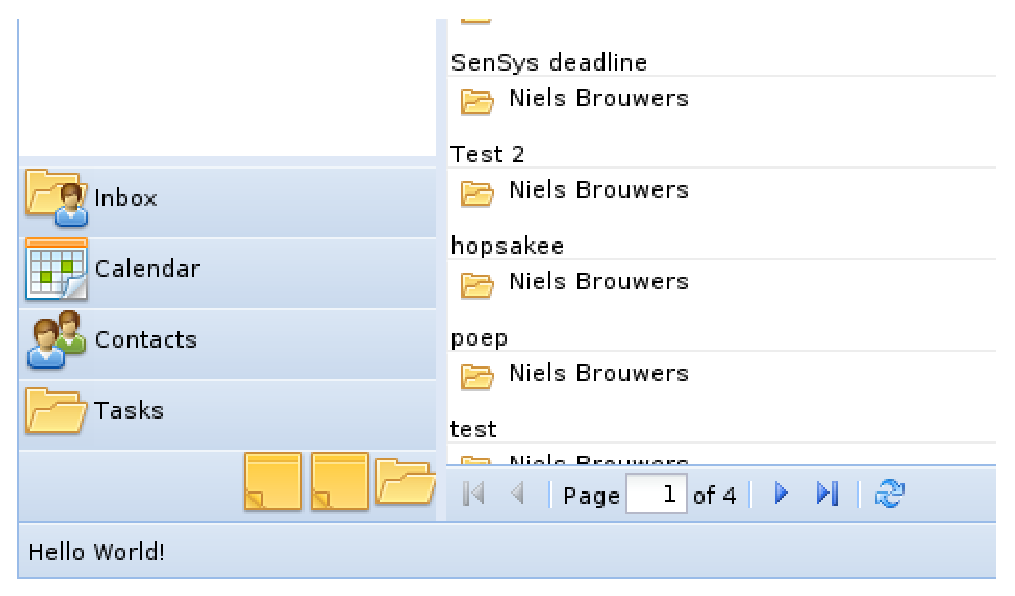
\includegraphics[width=9cm]{figures/plugin2.eps}
\caption{Folder status plugin.}
\label{figure:plugin2}
\end{figure}

Now that we have successfully added a UI component to the interface we would like it to show something
useful. We would like our plugin to display information about the folder that is currently selected.
The {\tt container} object has a {\tt folderselect} event that fires when the user selects a folder.
By listening for this event we can automatically update the text of our text item in the toolbar.

\begin{lstlisting}[caption={Attaching an event handler to the container.}, label=listing:plugin2]
init : function()
{
	this.registerInsertionPoint('statusbar.left', this.createFolderStatus, this);
	
	// Hook into the folder select event of the container
	container.on('folderselect', this.folderSelect, this);
},

updateFolderText : function(store, folder)
{
	// Set the text item text.
	this.textItem.setText(String.format("{0} items - {1} unread",
		folder.content_count,
		folder.content_unread
	));
},

folderSelect : function(store, folder)
{
	// Update the text item with the current store and folder.
	this.updateFolderText(store, folder);
},
\end{lstlisting}

The changed functions are shown in Listing \ref{listing:plugin2}. The event is hooked in {\tt init}, so that
{\tt folderSelect} is called when the user clicks a folder. This method in turn calls {\tt updateFolderText}
which updates the text on the toolbar text item.

The final touch to this plug-in is automatically updating the text when the contents of the folder change due
to user actions such the removal or creation of items. This is left as an exercise to the reader (hint: have
a look at Zarafa.HierarchyModel). The answer can be found in the implementation of 
{\tt Zarafa.plugins.FolderStatus}.

\section{A basic tasks context}
\label{section:taskscontext}

In this example we will build a tasks context. The context will be able to list tasks in a grid control.
We will start by creating a fresh new context called {\tt TaskContext} as shown in Listing 
\ref{listing:taskcontext1}.

Since a context is a type of plug-in the basic structure is similar to the plug-in described in Section
\ref{section:folderdetails}. There are three functions that are defined in the {\tt Context} class 
that every context must override. The {\tt bid} method implements the bidding scheme described in 
Section \ref{section:contexts}. The {\tt createContentPanel} and {\tt createToolbar} methods create 
the neccesairy UI components. 

The bidding function returns the numerical value 2 if the folder that is being selected is a tasks
folder, or -1 for any other. It checks this by looking at the 'container\_class' property of a folder. 
Since the built-in task context will bid 1 for task folders, our example implementation overrides it by 
bidding a higher value of 2. 

%\begin{itemize}
%	\item{{\tt bid(parameters:Object):Number} is used to bid on folders. See Section \ref{section:contexts}. } 
%	\item{{\tt createContentPanel():Ext.Panel} creates a content panel. } 
%	\item{{\tt createToolBar():Ext.Toolbar} creates a top tool bar. } 
%\end{itemize}

\begin{lstlisting}[caption={Boilerplate for a new context.}, label=listing:taskcontext1]
/**
 * @class Zarafa.ui.TaskContext
 * @extends Zarafa.ui.Context
 */
Zarafa.ui.TaskContext = function()
{
	var config = { name : 'taskcontext' };
	Zarafa.ui.TaskContext.superclass.constructor.call(this, config);
};

Ext.extend(Zarafa.ui.TaskContext, Zarafa.ui.Context, {
	
	// Bid on task folders.
	bid : function(parameters)
	{
	
		// Task folders containsitems of type IPF.Task
		if (parameters.folder.container_class=='IPF.Task') return 2;

		// return -1, don't handle this content type
		return -1;
	
	},
	
	// Create content panel.
	createContentPanel : function()
	{
		return new Ext.Panel({
			title : 'Hello World!',
			html : 'Hello World!'
		});
	},
	
	// Create tool bar.
	createToolbar : function()
	{
		return new Ext.Toolbar({
			items : 'Place holder.'
		});
	}	
	
});

container.registerPlugin(new Zarafa.ui.TaskContext());
\end{lstlisting}

Running this code will result in Figure \ref{figure:taskcontext}. When a tasks folder is selected the content
panel provided by the context will be shown, along with its tool bar. 

\begin{figure}[h!]
\centering
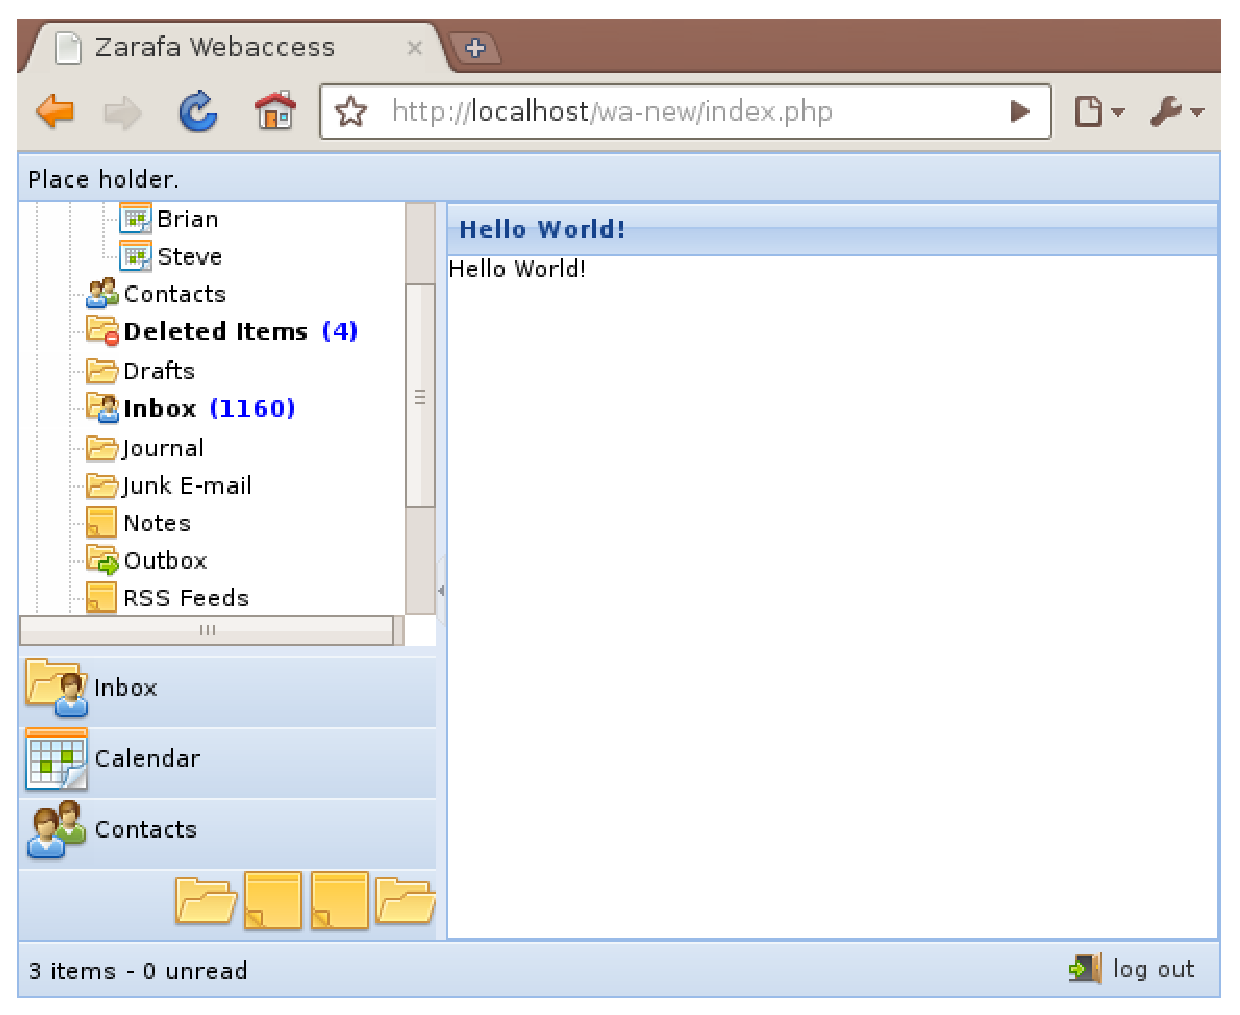
\includegraphics[width=9cm]{figures/taskcontext.eps}
\caption{Task context says hello.}
\label{figure:taskcontext}
\end{figure}

The next step is to retrieve tasks from the server and show them on screen. We do this by creating a grid panel
and attaching a store to it. Listing \ref{listing:taskcontext2} shows the modifed code. 

\begin{lstlisting}[caption={Adding a grid panel.}, label=listing:taskcontext2]
/**
 * @class Zarafa.ui.TaskContext
 * @extends Zarafa.ui.Context
 */
Zarafa.ui.TaskContext = function()
{
	var config = { name : 'taskcontext' };
	Zarafa.ui.TaskContext.superclass.constructor.call(this, config);
	
	// Convenience initialisation function.
	this.init();
};

Ext.extend(Zarafa.ui.TaskContext, Zarafa.ui.Context, {
	
	init : function()
	{
		// Create a store to hold our loaded task records.
		this.store = new Zarafa.comm.TaskStore();
	},
	
	// called when the context is enabled (the user clicks a task folder)
	enable : function(parameters)
	{
		this.store.load({
			storeId : parameters.store.id,
			entryId : parameters.folder.entryid
		});
	},
	
	// Create content panel.
	createContentPanel : function()
	{
		return new Ext.grid.GridPanel({
			border : false,
			
			viewConfig :
			{
				forceFit : true,
				showPreview : true,
				enableRowBody : true
			},

			// Column Model.
			cm : new Ext.grid.ColumnModel(
			[
				{
					dataIndex : 'owner',
					header : "Owner",
					sortable : true
				},
				{
					dataIndex : 'subject',
					header : "Subject",
					sortable : true
				}
			]),
            
			// Connect our store to the grid.
			store : this.store
		
		});
	},
	
	// bid() and createToolbar() omitted for brevity
	
});

container.registerPlugin(new Zarafa.ui.TaskContext());\end{lstlisting}

We first create an {\tt init} method that constructs a new instance of 
{\tt Zarafa.comm.TaskStore}. This is the store that will contain the task records displayed on the screen.
We want to load tasks into this store when a folder is selected by the user. To do this we
override the {\tt enable} method. It is automatically called by the framework when a context has
won the bidding round and just before its components are made visible. 
As with the {\tt bid} method, a parameter object is passed containing store and folder details.
We call {\tt load} on our store and pass it the MAPI ids of the store and folder so that it knows what to load.
Finally, to show the information to the user, we modify the {\tt createContentPanel} function to return a grid
panel, configured to show data from the store. 

\begin{figure}[h!]
\centering
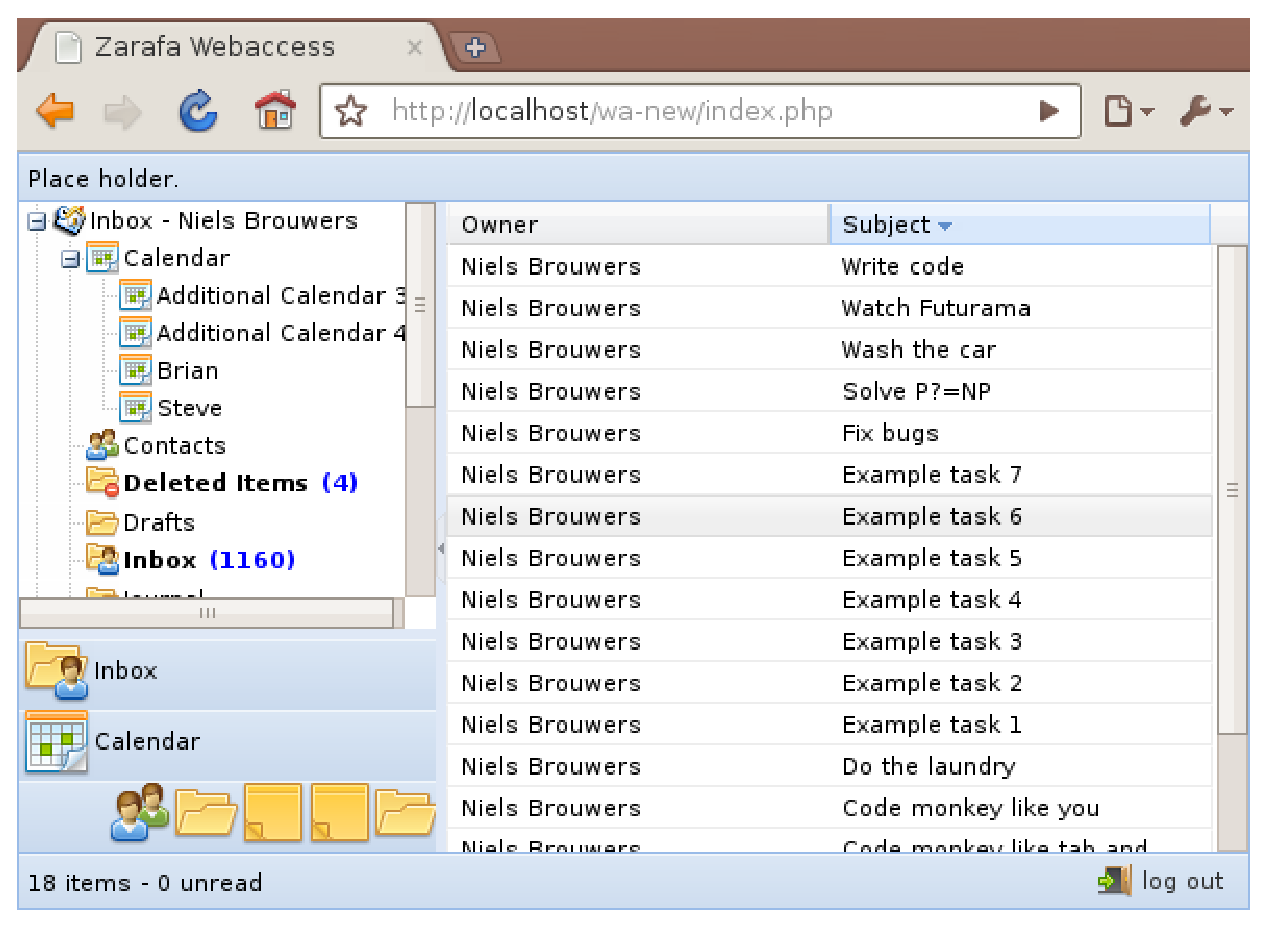
\includegraphics[width=9cm]{figures/taskcontext2.eps}
\caption{Task context with real data.}
\label{figure:taskcontext2}
\end{figure}

Figure \ref{figure:taskcontext2} shows the result. It is possible to sort by owner or subject by clicking the
corresponding column headers. The store will remember the store- and folder MAPI ids automatically, so that
subsequent load commands (in this case from the grid panel) collect the right data.

% \subsection{Adding a 'new' button}



	
\end{document}

